\chapter{\acl{hrc} System}
\label{chapter:hrc_system}

This chapter reviews the relevant hardware and software tools used during development and the software developed to support a practical implementation of action anticipation in human-robot collaboration.

\section{System Architecture \textcolor{red}{(LARCC, ROS-based framework)}}

The experimental part of this thesis was developed using the setup available at the Laboratory for Automation and Robotics (LAR) located in the Department of Mechanical Engineering at the University of Aveiro. This setup was designed to meet the requirements of the AUGMANITY mobilizing project\footnote{AUGMANITY website: \url{https://www.augmanity.pt}} and it contains an UR10e collaborative robot and multiple cameras.

\begin{figure}[h]
\centerline{\includegraphics[width=0.9\textwidth, trim={0 5cm 0 0}, clip]{figs/setup2.jpg}}
\caption[setup]{LAR hardware setup}
\label{fig:ur10e}
\end{figure}

\subsection{\acf{ros}}

\acs{ros}\cite{ROS2}\footnote{\acs{ros} 1 documentation: \url{https://wiki.ros.org}}\footnote{\acs{ros} 2 documentation: \url{https://docs.ros.org/en/humble}} is an open-source collection of tools and software libraries used to develop a robotics application and, in this work, it is used to establish communication throughout all of the infrastructure. ROS was chosen due to the hardware abstraction it offers given that it contains driver packages to deal with some hardware devices, allowing for easier communication with the robot and the cameras.
Other relevant features include:
\begin{itemize}
    \item \textbf{message broker}: every process in the project is a node in the \acs{ros} network and communicates with the other nodes mainly through topics (asynchronous publish/subscribe streaming of data) or services (synchronous RPC-style communication);
    \item \textbf{code reuse}: executables and packages are written to be as independent as possible, making the developer able to reuse them in another project;
    \item \textbf{rich ecosystem}: there are several open-source packages available to the developer that can be easily integrated;
    \item \textbf{scalability}: given that the nodes are so loosely coupled, it allows for node distribution;
    \item \textbf{language independence}: nodes can be written in any language since communication is established through well-defined objects;
    \item \textbf{data visualization}: there are tools to visualize the data and the functioning of the system in real-time, such as Rviz;
    \item \textbf{simulator support}: \acs{ros} has support for simulators with Gazebo being the most common.
\end{itemize}

For our system, the ROS 1 Noetic distribution was chosen over the more recent ROS 2 distributions so as to reuse work already done by other members of the AUGMANITY project at the University of Aveiro.

\subsection{Perception System \textcolor{red}{(Orbbec Astra Pro, OpenCV)}}
\label{subsection:perception_system}

%These are RGBD cameras developed by Orbbec Technologies, frequently used in computer vision and robotics for tasks such as face recognition, gesture recognition, human body tracking, three-dimensional measurement, environment perception, and three-dimensional map reconstruction\cite{AstraPro}.

In order to capture the necessary information from the environment, two Orbbec Astra Pro RGBD cameras were used. This camera model was developed by Orbbec Technologies and it is frequently used in computer vision and robotics\cite{AstraPro}. Among the available cameras, it was chosen since it allowed to capture both color and depth images.

\begin{figure}[h]
\centerline{\includegraphics[width=0.6\textwidth]{figs/Astra.jpg}}
\caption[Orbbec Astra Pro]{Orbbec Astra Pro \cite{AstraPro}}
\label{fig:orbbec_astra_pro}
\end{figure}

In the experimental setup, one of the cameras is placed above the workspace facing downwards allowing the perception of the objects in the table through the color image and the position of the user through the depth image. The second camera is above and slightly behind the robot to capture the user in front of the robot with the images from this camera being the ones used in the keypoint detection models. The communication with the cameras is established through ROS with the $usb\_cam$ package being used for the color image and the $ros\_astra\_camera$ package being used for the depth image. In order to have better control over the lightness in the environment, the back-light compensation was raised to the maximum in the $usb\_cam$ configurations. Then the frame rate was also set to 10 frames per second in both cameras given that those were enough frames for the following processing.

As said before, the color image of the first camera is used to detect objects in the environment. These objects are blocks of specific colors and therefore they can be identified with color segmentation, which is done with the help of OpenCV, a popular computer vision library. With this library, we start by cropping the image from the camera to a specific region of interest consisting of the table area, which is then converted from BGR to HSV given that the intervals of a color are easier to determine in this representation. From the HSV image and the color intervals, we obtain a mask for each color. These masks are then subject to a closing morphological operation to reduce any possible noise. Finally, the resulting areas are considered an object if they surpass a certain area threshold.

On the other hand, the depth image is used to obtain the position of the human in the workspace by cropping it to a certain region of interest and then detecting the highest point.

\subsection{Manipulator Arm Control \textcolor{red}{(UR10e cobot, Robotiq gripper, Moveit)}}
\label{subsection:manipulator_arm_control}

The collaborative robot available for this work is the UR10e. This robot model was developed by Universal Robots and it allows for payloads up to 12.5 kg and has a reach of 1300mm being suitable for tasks such as machine tending, palletizing, and packaging\cite{UR10e}. The one used in this work is equipped with a \textcolor{red}{(missing gripper model)} gripper.

\begin{figure}[h]
\centerline{\includegraphics[width=0.5\textwidth]{figs/UR10e.png}}
\caption[UR10e]{UR10e collaborative robot \cite{UR10e_image} \textcolor{red}{(missing gripper image)}}
\label{fig:ur10e}
\end{figure}

Both the robot and the gripper have ROS packages containing their drivers making their integration easier. The planning and execution of the arm movements are done trough the MoveIt\footnote{MoveIt documentation: \url{https://ros-planning.github.io/moveit_tutorials}} framework, which is a widely-used open-source framework for robotics applications involving motion planning, manipulation, 3D perception, kinematics, control, navigation, and collision checking, with OPML being chosen to handle the motion planning tasks.

The configurations of the drivers and MoveIt was already done by other members of the AUGMANITY project and can be found on Github\footnote{Github LarCC Repository: \url{https://github.com/afonsocastro/larcc_interface}} along with a higher-level API that encloses that logic. During this work, an additional feature to stop movements was added.

\subsection{Computational Systems \textcolor{red}{(DeepLAR, Computador Central, TensorFlow)}}

The tasks involved in this work, such as training deep-learning models and analyzing images in real time require high computational resources. To handle the real-time processing of images and robot control, the central computer present in the setup was used. To handle the deep-learning model training, the deep-learning research server from LAR was used, codenamed Deeplar:
\begin{itemize}
    \item AMD RyzenTM Threadripper 2950X;
    \item Four NVIDIA GEFORCE® RTX 2080 Ti;
    \item 128GB DDR4 RAM.
\end{itemize}

The model training in Deeplar is executed using docker images, which allows multiple people to use the computer with each having their own isolated training environment with their own dependencies. The images used to design and train machine learning models in this work are based on the latest TensorFlow official image for GPUs.

TensorFlow is one of the most popular machine learning frameworks along with Pytorch. In this work, the former was chosen over the latter since the higher-level API allowed for faster development. The main features of Tensorflow\footnote{Tensorflow documentation: \url{https://www.tensorflow.org/api_docs}} are:
\begin{itemize}
    \item \textbf{prepare data}: load data, data pre-processing and data augmentation;
    \item \textbf{build models}: design and train custom models with little code or use pre-trained ones (transfer learning);
    \item \textbf{deploy models}: helps using models in different platforms such as locally, in the cloud, in a browser, or in mobile;
    \item \textbf{implement MLOps}: run models in production, tracking their performance and identifying issues.
\end{itemize}

\section{Methodologies/Research Methods}

\subsection{Knowledge-Based Systems \textcolor{red}{(Experta)}}

\subsection{Keypoints Detection Frameworks \textcolor{red}{(OpenPose, OpenPifPaf, MediaPipe)}}
\label{subsection:keypointdetection}

This section reviews OpenPose and OpenPifPaf which are two projects containing models to detect key points in images, such as the human skeleton joints.

\subsubsection{OpenPose}

OpenPose\cite{Cao2021,Simon2017,Cao2018,Wei2016}\footnote{OpenPose documentation: \url{https://cmu-perceptual-computing-lab.github.io/openpose}} is an open-source project that aims to detect key points in the human body, face, hands, and feet from images. Its main features are:

\begin{itemize}
    \item 2D real-time key point detection based on the body/foot, the hand, or the face of multiple people;
    \item 3D real-time key point detection based on images from multiple cameras of one person;
    \item estimation of camera calibration parameters;
    \item single-person tracking.
\end{itemize}

OpenPose can be used through the command-line or using an API for Python or C++.

\begin{figure}[h]
\centerline{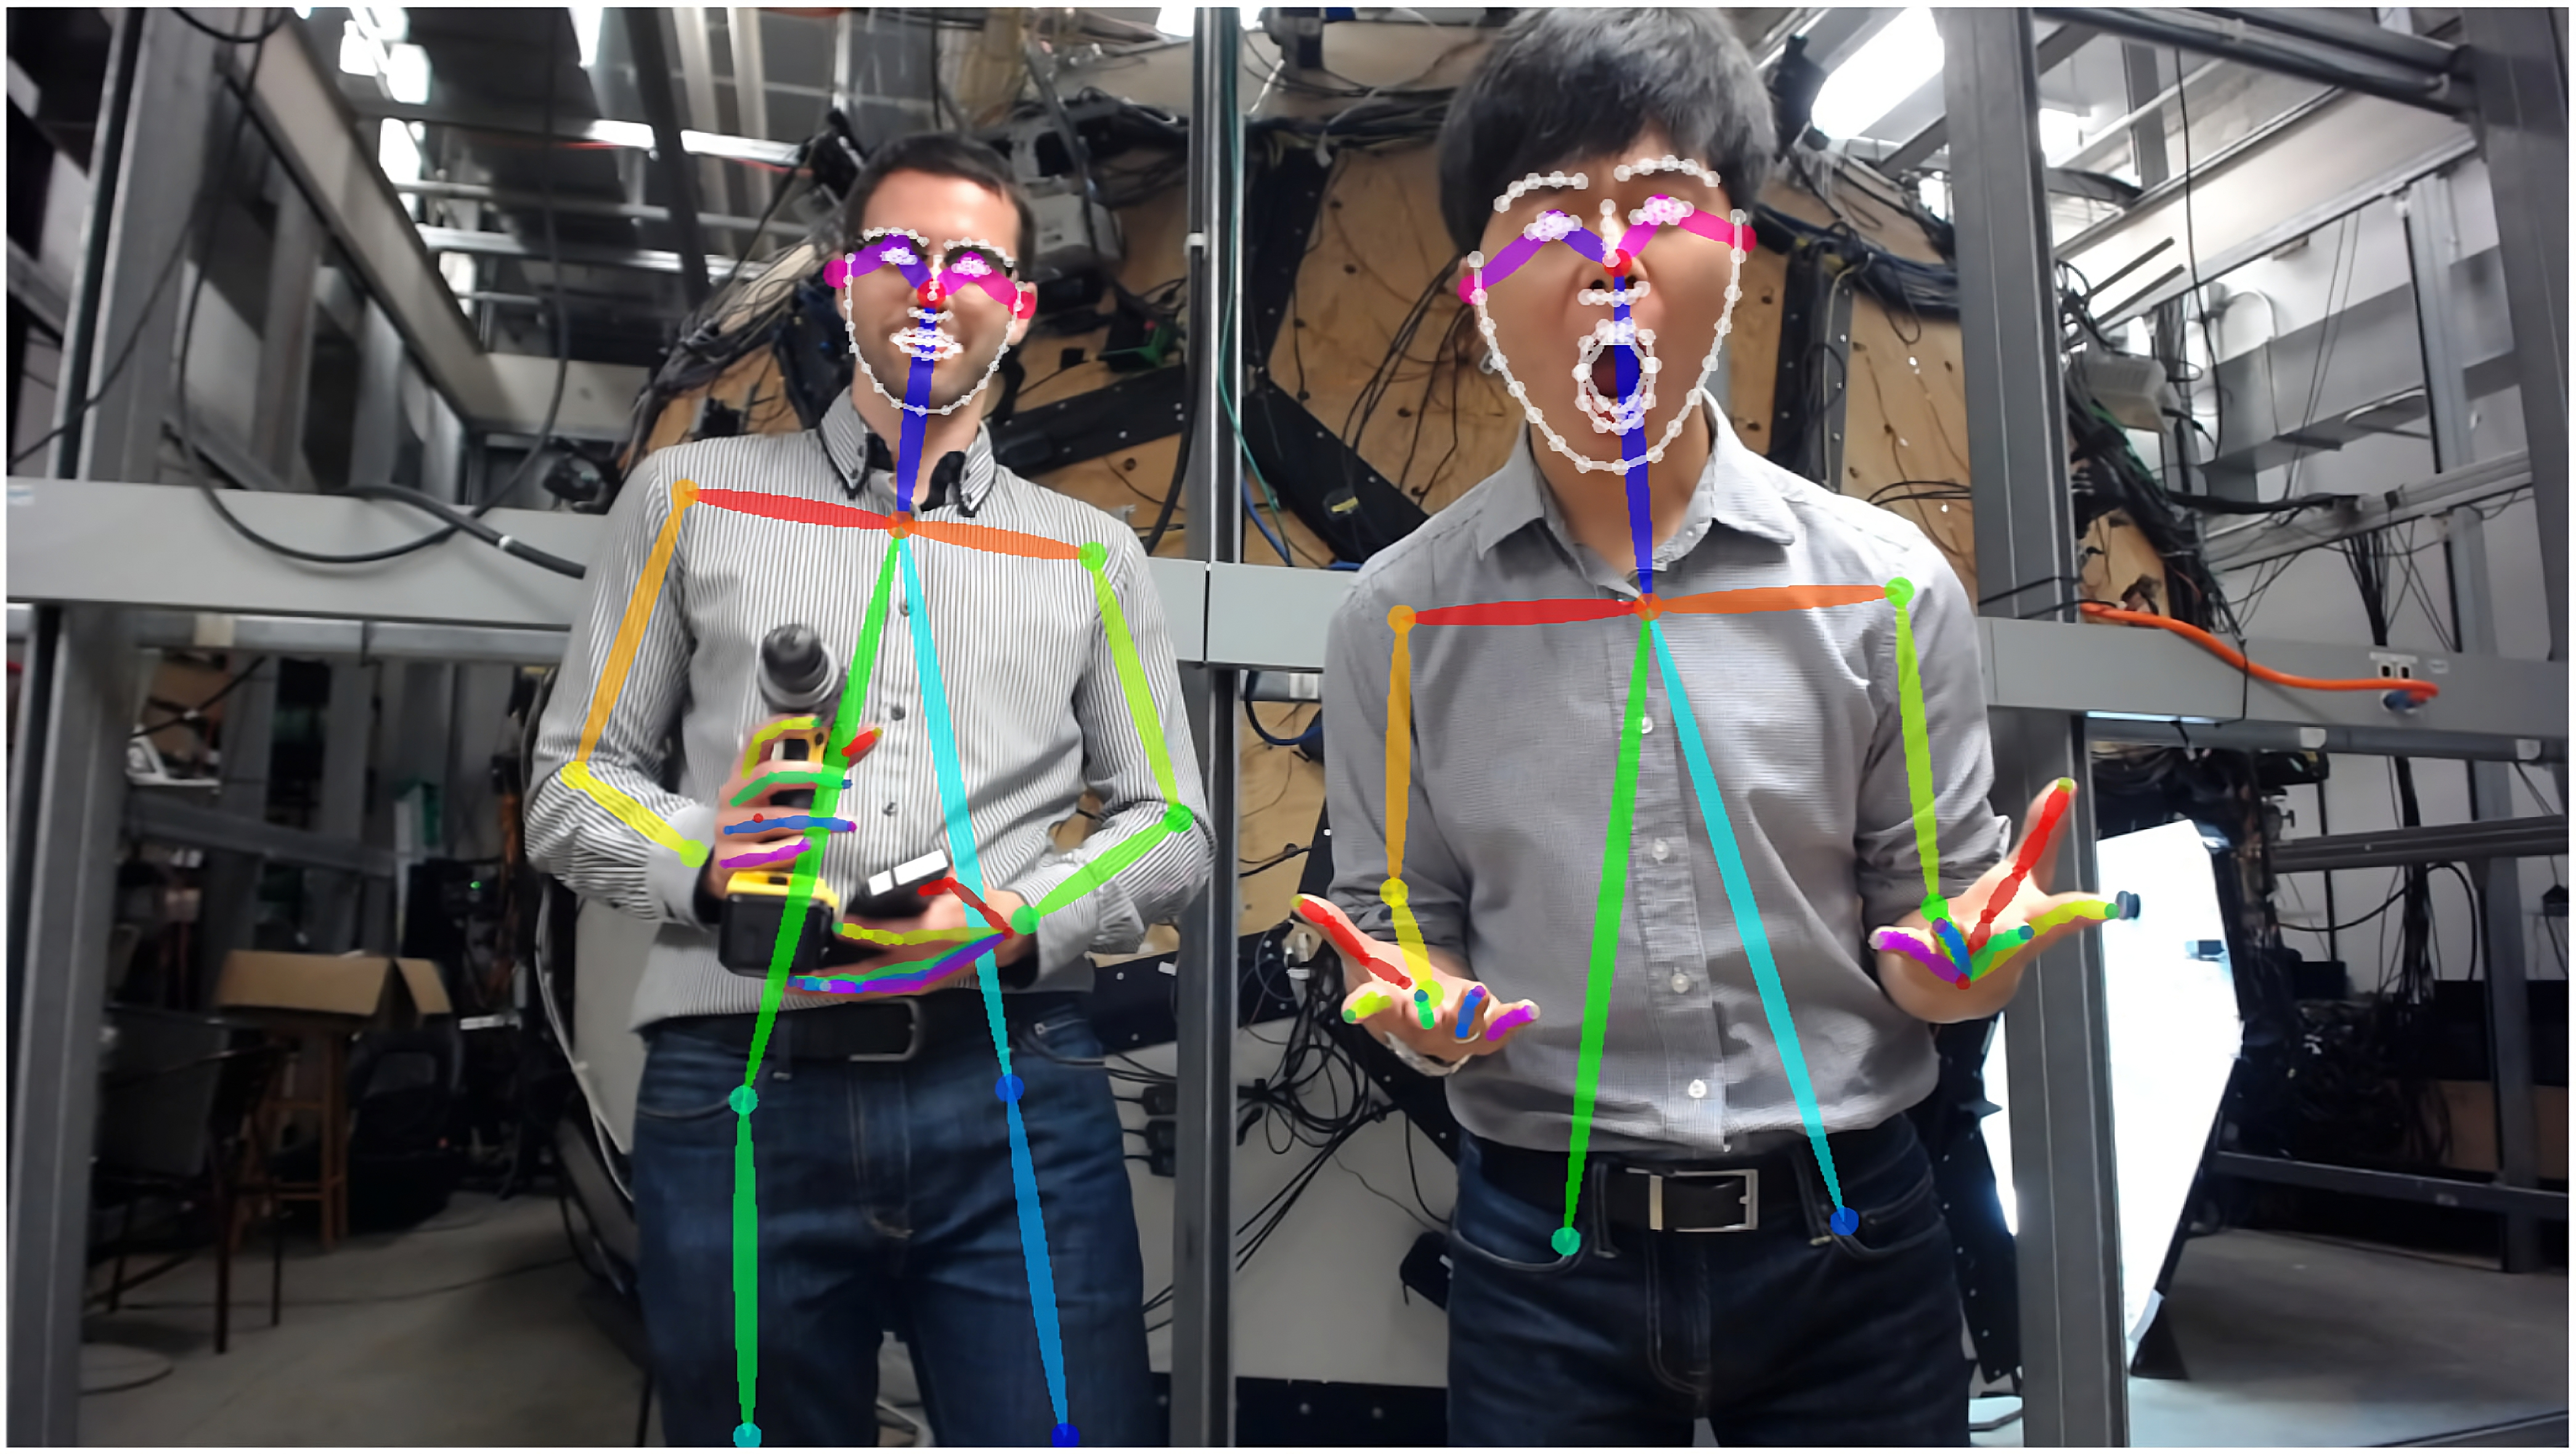
\includegraphics[height=1.55in]{figs/openpose.jpeg}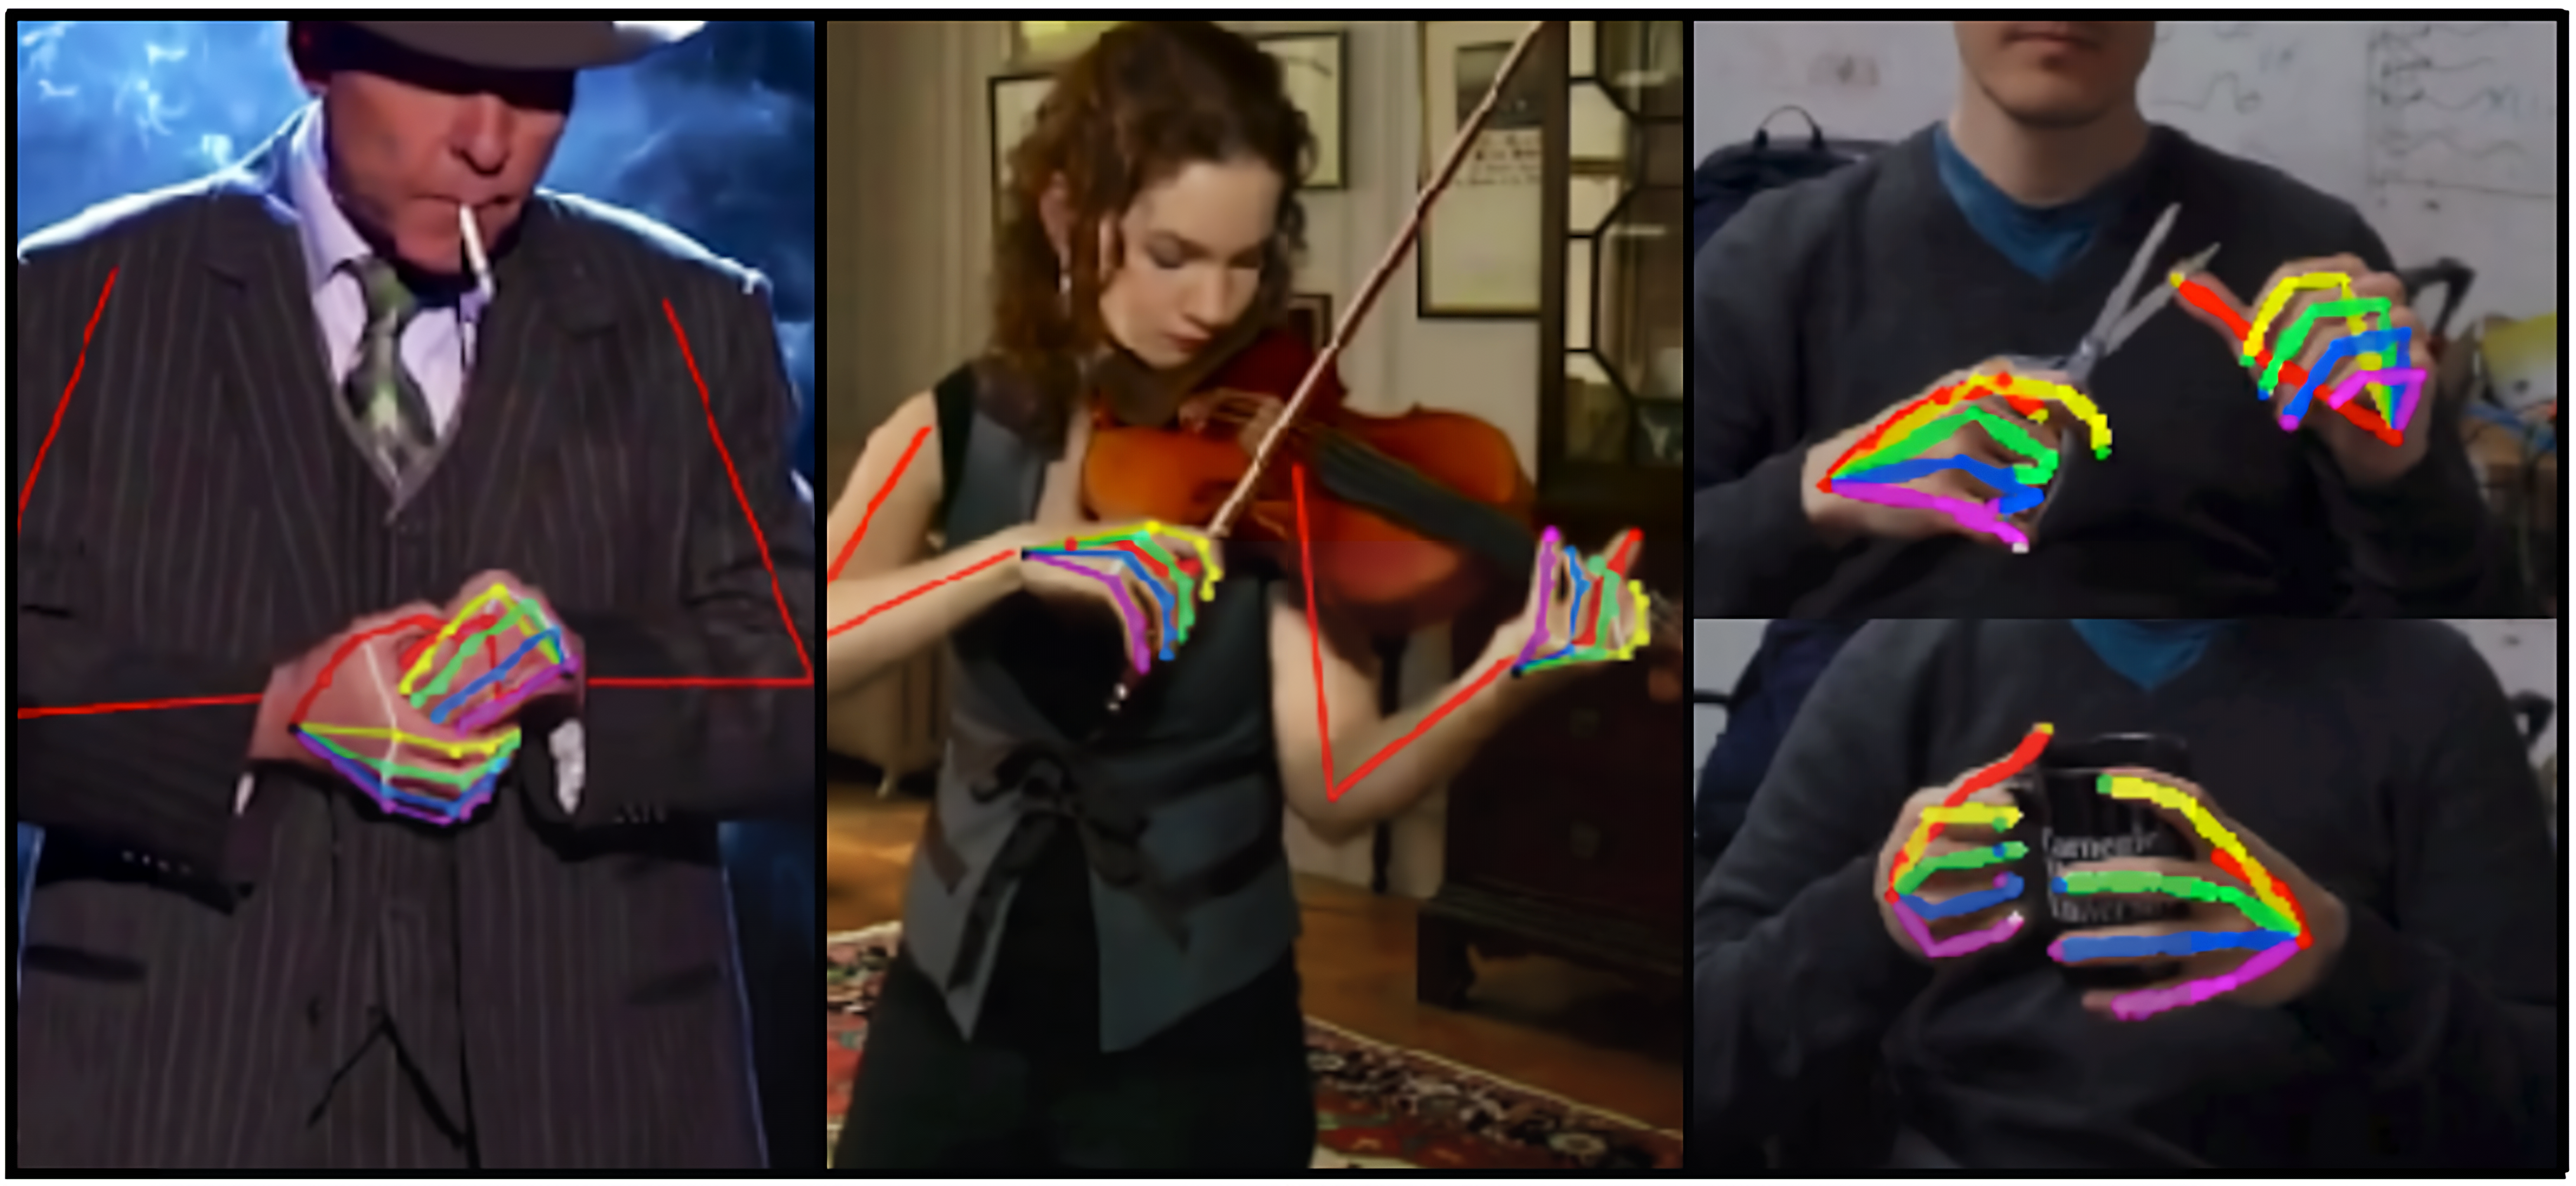
\includegraphics[height=1.55in]{figs/openpose2.PNG}}
\caption[OpenPose Examples]{OpenPose Examples \cite{Cao2021,Simon2017}}
\label{openpose}
\end{figure}

\subsubsection{OpenPifPaf}

OpenPifPaf\cite{Kreiss2021,Kreiss2019}\footnote{OpenPifPaf documentation: \url{https://openpifpaf.github.io}} is an open-source project that aims to detect, associate and track semantic key points. Detecting human joints is an example of its usage but it is also able to generalize this detection to other classes such as cars and animals. It can be installed as a python package which can then be imported.

\begin{figure}[h]
\centerline{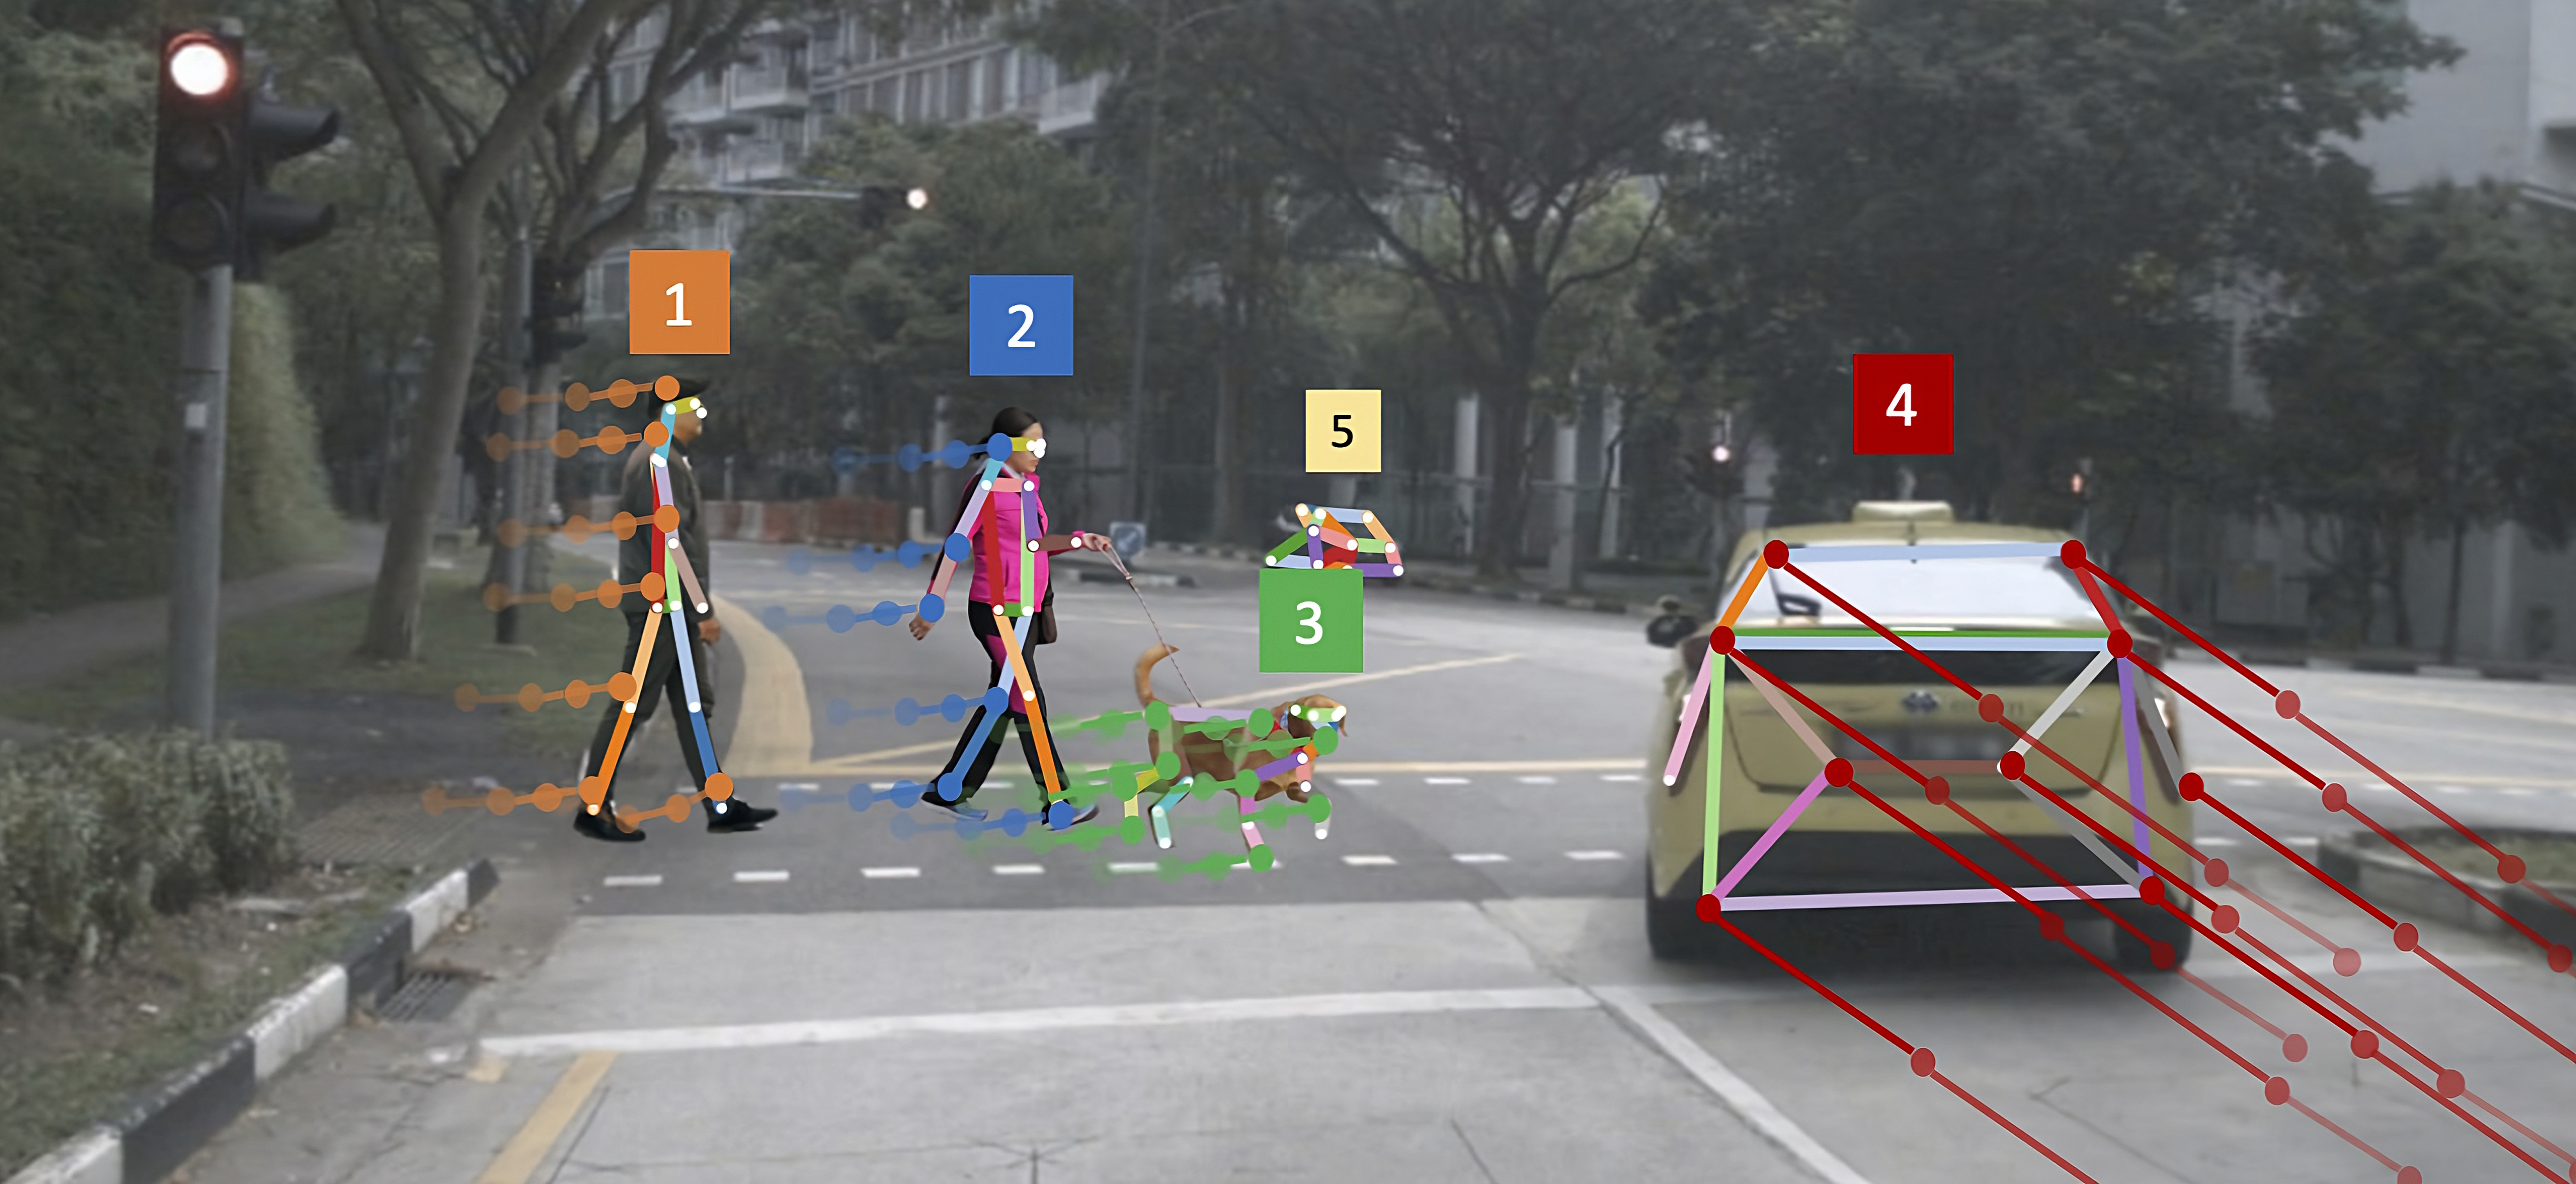
\includegraphics[height=1.8in]{figs/openpifpaf.jpeg}}
\caption[OpenPifPaf Example]{OpenPifPaf Example \cite{Kreiss2021}}
\label{openpifpaf}
\end{figure}

\subsubsection{MediaPipe}

\subsection{Convolutional Neural Networks}

\subsection{Transformer Neural Networks}
\label{subsection:transformer_neural_networks}

Transformer Neural Networks consist of a new kind of neural network architecture that aims to solve tasks involving sequence data such as those in natural language processing. They were initially proposed in the "Attention Is All You Need" paper published by Google Research in 2017\cite{Vaswani2017} and proceeded to surpass several established architectures in numerous tasks using attention mechanisms that identify complex relationships between elements in the input sequence.

According to \textcolor{red}{https://learning.oreilly.com/library/view/deep-learning-with/9781803232911/}, the transformer's architectures are built upon 4 core concepts: positional encoding, attention, self-attention, and multi-head (self-)attention.

\subsubsection{Positional encoding}

RNNs are able to work with sequences given that the tokens are processed sequentially. However, this approach comes with the disadvantage of the model having greater difficulty in analyzing long sequences, since important data might be forgotten. Transformers address this issue by using positional encoding, assigning a unique number to each token representing its position in the input sequence. This enables the transformer to learn the significance of each token's position.

\subsubsection{Attention}

Attention is a concept that consists in measuring the relative importance of the input tokens to the output tokens. It was initially designed to facilitate language translation given that, when translating text from one language to the other, each word in the output can be influenced by multiple words from the input, and it became a key idea behind the transformer's architecture.

\subsubsection{Self-attention}

Self-attention derives from attention but consists in measuring the relative importance of the input tokens to the other tokens of the input sequence instead of the output tokens. This concept allows the model to learn the relationships between tokens and their relevance in the input sequence even if they are far away.
 
\subsubsection{Multi-head (self-)attention}

Multi-head (self-)attention refers to the fact that a transformer can have multiple attention heads. Each attention head performs a parallel process of (self-)attention allowing for multiple resulting weight matrices and, therefore, multiple definitions of relevance between the tokens.

\subsubsection{Architecture}

\begin{figure}[h]
\centerline{\includegraphics[height=6in]{figs/transformer.jpg}}
\caption[Transformer Architecture]{Transformer Architecture \cite{Vaswani2017}}
\label{fig:transformer_arch}
\end{figure}

\section{Integration of First Anticipation Experiments}

This section covers the implementation of the human-robot collaboration infrastructure that will serve as a base for an anticipation application and the first anticipation experiments realized to validate it.

\subsection{Assembly Task: Build a Three-Color Flag \textcolor{red}{(Problem description: interaction experiment and focus on integration...)}}

To develop the necessary infrastructure, a concrete problem was needed. For this work, it was chosen to use sequences of big \textcolor{red}{"Lego"} blocks comparable to the stripes of a flag, as shown in Fig~\ref{fig:flags_examples}.

\begin{figure}[H]%[!ht]
    \centering
    \begin{tikzpicture}[>=latex']

    \node (france_flag) {\includegraphics[width=.2\textwidth]{figs/France.png}};
    \node[right =2cm of france_flag] (france_blocks) {\includegraphics[width=.2\textwidth]{figs/flag1.jpg}};
    \node[below =0.3cm of france_flag] (portugal_flag) {\includegraphics[width=.2\textwidth]{figs/Portugal.png}};
    \node[right =2cm of portugal_flag] (portugal_blocks) {\includegraphics[width=.2\textwidth]{figs/flag2.jpg}};

    \path[draw, ->, text width=2cm, align=center]
        (france_flag) edge (france_blocks)
        (portugal_flag) edge (portugal_blocks)
    ;
    
\end{tikzpicture}
    \caption{Flags Examples}
    \label{fig:flags_examples}
\end{figure}

These blocks are initially placed behind the robot, and the robot must fetch them and place them next to the user so that the user can build a flag. The blocks must be fetched in a certain order and there must be a way for the user to tell the robot that it is fetching the wrong block.

\textcolor{red}{missing workspace image from above}

Before the anticipation experiments, a base infrastructure was developed to build upon, integrating the perception system described in Subsection \ref{subsection:perception_system} and the manipulator arm control system described in Subsection \ref{subsection:manipulator_arm_control}. Connecting both of them is a decision-making node as shown in Fig~\ref{}. The logic in this node is implemented through a state machine with the behavior in each state corresponding to a method of a class, which facilitates the integration of additional logic by using subclasses of that class.

The initial decision-making logic developed relied on interactions between the robot and the user. When the user puts his hand above a small block, if the robot is idle, then it proceeds to fetch a block of the same color. Additionally, when the user hovers his hand over the violet block while the robot is fetching a block, it means that the robot is fetching the wrong block, so it must stop and put the block back where it was before if it was already picked up. These interactions are also the fallback behavior if the methods in the following experiments fail to anticipate the block that the user desires.

\subsubsection{State Machine Logic}

As said before, the decision making node contains an internal state machine. Although the logic of some states changes depending on the solution, all implementations follow the same general design represented in the state machine diagram shown in Fig.~\ref{fig:state_machine}.

\begin{figure}[H]%[!ht]
    \centering
    \begin{tikzpicture}[
        > = stealth, % arrow head style
        shorten > = 1pt, % don't touch arrow head to node
        auto,
        node distance = 3.8cm, % distance between nodes
        thick % line style
    ]
    
    \tikzstyle{every state}=[
        draw = black,
        thick,
        fill = white,
        minimum size = 4mm,
        text width = 1.5cm,
        align = center
    ]
    
    \node[state] (idle) at (0,0) {idle};
    \node[state] (picking_up) [right of=idle] {picking up};
    \node[state] (moving_closer) [right of=picking_up] {moving closer};
    \node[state] (putting_down) [below of=picking_up] {putting down};
    \node[state] (stop_side_switch) [right of=moving_closer] {stop side switch};
    \node[state] (stop_wrong_guess) [above of=picking_up] {stop wrong guess};

    \path[every edge,
    	->,
    	text width=1.8cm,
    	align=center
    	]
    (idle)             edge             node {knows which block is the next}        (picking_up)
    (picking_up)       edge             node {object picked up}                     (moving_closer)
    (moving_closer)    edge[bend left]  node {robot in put down position}           (putting_down)
    (putting_down)     edge[bend left]  node {robot retreated}                      (idle)
    (moving_closer)    edge[bend left]  node {user changed side}                    (stop_side_switch)
    (stop_side_switch) edge[bend left]  node {robot stopped}                        (moving_closer)
    (picking_up)       edge             node[right] {wrong assembly sequence}       (stop_wrong_guess)
    (moving_closer)    edge[bend right] node[above right] {wrong assembly sequence} (stop_wrong_guess)
    (stop_wrong_guess) edge[bend right] node[above left] {reverted previous guess}  (idle)
    ;

\end{tikzpicture}
    \caption{State Machine}
    \label{fig:state_machine}
\end{figure}

\begin{itemize}
    \item \textbf{idle}: State corresponding to when the robot does not know which is the next block. If the sequence has not started yet then it waits for the user to choose the first block and then the state changes to $picking$ $up$. If the sequence has already started then the database is fetched for the possible next blocks and then if at least one block is returned the state changes to $picking$ $up$ or if none is returned the system waits for the user to choose the next block.
    \item \textbf{picking up}: State corresponding to while the robot is picking up a certain block. After it picks it up the state changes to $moving$ $closer$ unless it was picking the wrong object in which case it changes to $stop$ $wrong$ $guess$.
    \item \textbf{moving closer}: State corresponding to the movement until the put-down position opposite to the user so that the robot does not constrain him. After the robot reaches the put-down position the state changes to $putting$ $down$. If the robot is holding the wrong object then the state changes to $stop$ $wrong$ $guess$ instead and if the user changes side the state changes to $stop$ $side$ $switch$.
    \item \textbf{putting down}: State corresponding to the movement necessary to put down the block in the table and the retreat of the robot outside the user's workspace. After that, the state changes to $idle$.
    \item \textbf{stop side switch}: State corresponding to the action of stopping the robot because the user changed sides. After the robot is stopped the state changes back to $moving$ $closer$.
    \item \textbf{stop wrong guess}: State corresponding to the action of stopping the robot because the user indicated that it was the wrong block. If the robot was already holding a block then that block is put back where it was while in this state. After the robot is stopped and it is not holding a block the state changes to $picking$ $up$ if there are still more possible blocks in the database. Otherwise, the state changes to $idle$ so that it waits for a user request.
\end{itemize}

\subsection{First Anticipation Experiments \textcolor{red}{(probabilities, rule-based \& rule-based + MediaPipe)}}

This subsection covers the workflow of the different experiments realized.

\subsubsection{Probability Based}

The first experiment consisted in having a database of probabilities that the robot would check to anticipate the block that the user would need next. These probabilities were established according to the possible country flags. However, the first block is still requested by the user and, if the robot exhausts all possibilities that it knows of, the user is able to request the following block using the interactions described in the first solution.

\subsubsection{Rule Based}

\textcolor{red}{...}

\subsubsection{Rule Based + MediaPipe}

\textcolor{red}{...}

\if{0}
\subsection{System ROS Architecture}

The communication between the robot, the sensors, and the programming logic is established using Robot Operating System (ROS) with the following 5 main nodes.

\textcolor{red}{a diagram might be a good idea to better visualize the solution}

\subsubsection{orbbec\_camera}

This node is responsible for receiving the color and depth images from the Orbbec camera and publishing them on ROS. In order to control to have better control over the lightness in the environment, the back-light compensation was raised to the maximum.

\subsubsection{human\_locator}

This node is responsible for analyzing the depth images and returning the position of the highest point in a certain region of interest which is then considered as the position of the human in the workspace.

\subsubsection{object\_color\_segmenter}

This node is responsible for analyzing the color images and returning the position of the objects in the workspace using color segmentation.

\subsubsection{decision\_making\_block}

This node is responsible for receiving the information resulting from the sensor data and keeping an internal state machine to decide what actions should be taken and when they should be taken.

\subsubsection{move\_it!}

This is a group of nodes responsible for planning the robot's trajectory in each action.
\fi

\section{Final Remarks}